\documentclass[11pt,a4paper]{article}

% -- Packages ------------------------------------------------------------------
\usepackage[T1]{fontenc}
\usepackage[utf8]{inputenc}
\usepackage[english]{babel}
\usepackage{lmodern}
\usepackage{microtype}
\usepackage{geometry}
\geometry{margin=25mm}

\usepackage{amsmath,amssymb,bm}
\usepackage{mathtools}
\usepackage{siunitx}
\sisetup{per-mode=symbol, detect-all}

\usepackage{booktabs}
\usepackage{array}
\usepackage{multirow}

\usepackage{graphicx}
\usepackage{tikz}
\usetikzlibrary{shapes.geometric, arrows.meta, positioning, calc, fit, backgrounds}
\usepackage{pgfplots}
\pgfplotsset{compat=1.18}

\usepackage{listings}
\usepackage{xcolor}
\usepackage{hyperref}
\hypersetup{colorlinks=true, linkcolor=blue!60!black, citecolor=green!50!black,
            urlcolor=blue!80!black}

\usepackage{caption}
\captionsetup{font=small, labelfont=bf}

% -- Custom colours -------------------------------------------------------------
\definecolor{codeblue}{RGB}{0,70,140}
\definecolor{codegray}{RGB}{100,100,100}
\definecolor{codegreen}{RGB}{0,120,60}
\definecolor{codeback}{RGB}{248,248,248}

% -- Listings style -------------------------------------------------------------
\lstdefinestyle{verilog}{
  language=Verilog,
  backgroundcolor=\color{codeback},
  basicstyle=\ttfamily\scriptsize, % \small, \footnotesize, \scriptsize,  \tiny
  keywordstyle=\color{codeblue}\bfseries,
  commentstyle=\color{codegreen}\itshape,
  stringstyle=\color{orange!80!black},
  numberstyle=\tiny\color{codegray},
  numbers=left,
  stepnumber=1,
  frame=single,
  framerule=0.4pt,
  rulecolor=\color{gray!40},
  breaklines=true,
  tabsize=4,
  showstringspaces=false
}


% -- Macros ---------------------------------------------------------------------
\newcommand{\Ts}{T_{\mathrm{s}}}
\newcommand{\vdc}{V_{\mathrm{dc}}}
\newcommand{\iref}{\bm{i}^{*}}
\newcommand{\ipred}{\hat{\bm{i}}}
\newcommand{\sa}{S_{\mathrm{a}}}
\newcommand{\Sb}{S_{\mathrm{b}}}
\newcommand{\Sc}{S_{\mathrm{c}}}

% ══════════════════════════════════════════════════════════════════════════════
\begin{document}

\title{\textbf{Finite Control Set Model Predictive Control\\
for a Three-Level T-Type Inverter\\
\large FPGA Implementation on Xilinx Zynq-7000}}
\author{Davide}
\date{\today}
\maketitle
\tableofcontents
\bigskip\hrule\bigskip

% ══════════════════════════════════════════════════════════════════════════════
\section{Introduction}
\label{sec:intro}

Three-level T-type inverters are widely adopted in medium-power drives and
grid-tied converters because they combine the low switching losses of
two-level topologies with the improved harmonic spectrum of NPC
structures~\cite{kolar2010ttype}.  Finite Control Set Model Predictive
Control (FCS-MPC) is a natural fit for FPGA implementation: it enumerates
a finite number of switching states, evaluates a cost function for each,
and selects the optimal one within a single sampling period.

This document covers:
\begin{enumerate}
  \item T-type inverter model and state equations (\S\,\ref{sec:model});
  \item Cost function, one-step prediction horizon, and current tracking
        (\S\,\ref{sec:mpc});
  \item Single-IGBT switching constraint (\S\,\ref{sec:constraint});
  \item AXI4-Lite interface for current reference and ADC readback
        (\S\,\ref{sec:axi});
  \item RTL block diagram and Verilog architecture for Zynq-7000
        (\S\,\ref{sec:rtl}).
\end{enumerate}

% ══════════════════════════════════════════════════════════════════════════════
\section{T-Type Inverter Model and State Equations}
\label{sec:model}

\subsection{Topology}
\label{sec:topo}

The three-level T-type inverter (Fig.\,\ref{fig:ttopo}) uses, per phase
$x\in\{a,b,c\}$, four IGBTs:
\begin{itemize}
  \item $T_{x1}$, $T_{x4}$ -- outer devices, connected to $+\vdc/2$ and
        $-\vdc/2$;
  \item $T_{x2}$, $T_{x3}$ -- inner bidirectional switch to the neutral
        point~NP.
\end{itemize}

Each phase can produce three voltage levels:
\begin{equation}
  v_{xN} \in \left\{+\tfrac{\vdc}{2},\ 0,\ -\tfrac{\vdc}{2}\right\}
  \triangleq \left\{P,\ O,\ N\right\}
\end{equation}
The switching state per phase is encoded as $s_x \in \{+1, 0, -1\}$, so
the phase-to-neutral-point voltage is:
\begin{equation}
  v_{xN} = s_x\,\frac{\vdc}{2}, \qquad s_x \in \{-1,0,+1\}.
  \label{eq:vxN}
\end{equation}

\begin{figure}[htbp]
  \centering
  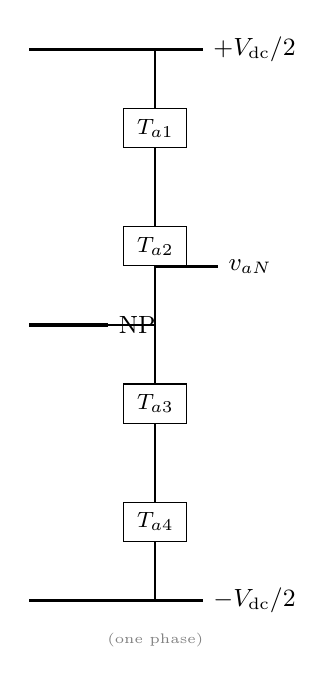
\begin{tikzpicture}[
      igbt/.style={rectangle, draw, minimum width=8mm, minimum height=5mm,
                   font=\footnotesize},
      bus/.style={very thick},
      wire/.style={thick},
      >=Stealth]
    % DC bus rails
    \draw[bus] (0,3.5) -- (2.2,3.5) node[right]{\small $+\vdc/2$};
    \draw[bus] (0,-3.5) -- (2.2,-3.5) node[right]{\small $-\vdc/2$};
    \draw[bus] (0,0) -- (1.0,0) node[right]{\small NP};
    % IGBTs (one phase shown)
    \node[igbt] (T1) at (1.6, 2.5) {$T_{a1}$};
    \node[igbt] (T2) at (1.6, 1.0) {$T_{a2}$};
    \node[igbt] (T3) at (1.6,-1.0) {$T_{a3}$};
    \node[igbt] (T4) at (1.6,-2.5) {$T_{a4}$};
    % Connections
    \draw[wire] (1.6,3.5) -- (T1.north);
    \draw[wire] (T1.south) -- (T2.north);
    \draw[wire] (T2.south) -- (T3.north);
    \draw[wire] (T3.south) -- (T4.north);
    \draw[wire] (T4.south) -- (1.6,-3.5);
    % Output node
    \draw[wire] (T2.south) -- ++(0.8,0) node[right]{\small $v_{aN}$};
    % NP connection
    \draw[wire] (1.0,0) -- (T2.south|-0,0) -- (T2.south|-0,0);
    \draw[wire,dashed] (1.0,0) -- (1.3,0) -- (1.3,0) -- (T2.south|-1.3,0);
    \node[font=\tiny,gray] at (1.6,-4) {(one phase)};
  \end{tikzpicture}
  \caption{Schematic of one phase of the T-type three-level inverter.
           $T_{a2}$--$T_{a3}$ form the bidirectional neutral-point switch.}
  \label{fig:ttopo}
\end{figure}

\subsection{Valid Switching States per Phase}
\label{sec:states}

Table\,\ref{tab:states} lists the four IGBT states for each output level.

\begin{table}[htbp]
  \centering
  \caption{T-type switching states per phase ($x\in\{a,b,c\}$).}
  \label{tab:states}
  \begin{tabular}{cccccl}
    \toprule
    $s_x$ & Level & $T_{x1}$ & $T_{x2}$ & $T_{x3}$ & $T_{x4}$ \\
    \midrule
    $+1$ & P & ON  & ON  & OFF & OFF \\
    $ 0$ & O & OFF & ON  & ON  & OFF \\
    $-1$ & N & OFF & OFF & ON  & ON  \\
    \bottomrule
  \end{tabular}
\end{table}

The three-phase system has $3^3 = 27$ voltage vectors $\bm{v}_k
= (s_a,s_b,s_c)$.

\subsection{RL-Load State Equations}
\label{sec:rl}

The load is modelled as a series RL branch (motor equivalent, or filter
inductor).  The line-to-line voltages are:
\begin{equation}
  v_{ab} = v_{aN} - v_{bN}, \quad
  v_{bc} = v_{bN} - v_{cN}, \quad
  v_{ca} = v_{cN} - v_{aN}.
\end{equation}
The phase voltage referred to the star point is:
\begin{equation}
  v_{xs} = v_{xN} - v_{ns}, \quad
  v_{ns} = \tfrac{1}{3}(v_{aN}+v_{bN}+v_{cN}).
\end{equation}
The continuous-time state equation for phase current $i_x$ is:
\begin{equation}
  L\,\frac{d i_x}{dt} = v_{xs} - R\,i_x - e_x,
  \label{eq:ct}
\end{equation}
where $e_x$ is the back-EMF (or grid voltage).  In matrix form with
$\bm{i} = [i_a,i_b,i_c]^{\top}$:
\begin{equation}
  \dot{\bm{i}} = -\frac{R}{L}\bm{i} + \frac{1}{L}\bm{v}_s - \frac{1}{L}\bm{e},
  \label{eq:ss}
\end{equation}
where $\bm{v}_s = \mathbf{T}\bm{v}_N$ with the Clarke matrix
\begin{equation}
  \mathbf{T} = \frac{1}{3}\begin{bmatrix}
    2 & -1 & -1 \\ -1 & 2 & -1 \\ -1 & -1 & 2
  \end{bmatrix}.
\end{equation}

\subsection{Discrete-Time Prediction Model}
\label{sec:disc}

Forward Euler discretisation with sampling period $\Ts$:
\begin{equation}
  \bm{i}(k+1) = \left(1 - \frac{R\Ts}{L}\right)\bm{i}(k)
               + \frac{\Ts}{L}\left[\bm{v}_s(k) - \bm{e}(k)\right].
  \label{eq:disc}
\end{equation}
For FPGA implementation~\eqref{eq:disc} is evaluated in fixed-point
arithmetic; the coefficients $\alpha = 1 - R\Ts/L$ and $\beta = \Ts/L$
are pre-computed and stored as $Q_{16}$ constants.

% ══════════════════════════════════════════════════════════════════════════════
\section{Cost Function and FCS-MPC Prediction}
\label{sec:mpc}

\subsection{Algorithm Overview}
\label{sec:algo}

At every sampling instant $k$ the FCS-MPC algorithm:
\begin{enumerate}
  \item Reads the measured currents $\bm{i}(k)$ from the ADC;
  \item Reads the current reference $\iref(k)$ from the AXI register;
  \item Enumerates all 27 candidate vectors $\bm{v}_j$, $j=0,\ldots,26$;
  \item Applies the constraint of \S\,\ref{sec:constraint} to retain only
        admissible vectors;
  \item For each admissible vector, predicts $\ipred_j(k+1)$ via
        \eqref{eq:disc};
  \item Evaluates the cost function $g_j$;
  \item Applies the switching state $\bm{u}^* = \arg\min_j g_j$.
\end{enumerate}

\subsection{Cost Function}
\label{sec:cost}

The primary term penalises the current tracking error:
\begin{equation}
  g_j = \left\|\iref(k+1) - \ipred_j(k+1)\right\|^2
      = \sum_{x \in \{a,b,c\}}
        \left(i_x^*(k+1) - \hat{i}_{x,j}(k+1)\right)^2.
  \label{eq:cost}
\end{equation}
An optional switching frequency reduction term can be added:
\begin{equation}
  g_j^{\mathrm{ext}} = g_j + \lambda_{\Delta u}\,\Delta n_j,
  \label{eq:costext}
\end{equation}
where $\Delta n_j$ is the total number of IGBT commutations required to
move from the current switching state to candidate $j$, and
$\lambda_{\Delta u} \geq 0$ is a tunable penalty weight.

\subsection{One-Step Prediction Horizon}
\label{sec:horizon}

The prediction horizon is $N_p = 1$.  The reference at $k+1$ is
extrapolated as $\iref(k+1) \approx 2\iref(k) - \iref(k-1)$ (first-order
hold), which requires storing the previous reference sample.

% ══════════════════════════════════════════════════════════════════════════════
\section{Single-IGBT Switching Constraint}
\label{sec:constraint}

\subsection{Motivation}
\label{sec:constr_mot}

Switching multiple IGBTs simultaneously within one sampling period
increases switching losses and can excite high-frequency resonances in the
DC-link capacitors.  The constraint limits the number of \emph{device}
transitions per sampling interval to at most one per phase, and
specifically to a single device commutation across all three phases.

\subsection{Transition Graph}
\label{sec:graph}

For each phase the allowed transitions are:
\begin{equation}
  \Delta s_x = s_x(k+1) - s_x(k) \in \{-1,\, 0,\, +1\}.
\end{equation}
Jumping from $s_x = +1$ to $s_x = -1$ (or vice versa) in one step
requires two device transitions (e.g.\ $T_{x1}$ OFF and $T_{x4}$ ON),
which is \emph{forbidden}.

The set of admissible vectors at step $k$ given current state
$\bm{s}(k)$ is:
\begin{equation}
  \mathcal{U}(k) = \left\{ \bm{s} \in \{-1,0,+1\}^3 \;\middle|\;
    \sum_{x} \mathbb{1}\bigl[s_x \neq s_x(k)\bigr] \leq 1
    \;\;\text{and}\;\;
    |s_x - s_x(k)| \leq 1 \;\forall\,x \right\}.
  \label{eq:admissible}
\end{equation}
This yields at most $1 + 3\times 2 = 7$ admissible states from any
interior point, reducing the enumeration from 27 to at most 7 candidates.

\subsection{IGBT-Level Decoding}
\label{sec:decode}

Once the optimal $s_x^*$ is determined, the gate signals are decoded
according to Table\,\ref{tab:states}.  The transition logic per phase is:
\begin{itemize}
  \item $s_x: 0 \to +1$: turn ON $T_{x1}$ (one commutation);
  \item $s_x: +1 \to 0$: turn OFF $T_{x1}$ (one commutation);
  \item $s_x: 0 \to -1$: turn ON $T_{x4}$ (one commutation);
  \item $s_x: -1 \to 0$: turn OFF $T_{x4}$ (one commutation).
\end{itemize}
Transitions $\pm 1 \to \mp 1$ are blocked by the constraint.

% ══════════════════════════════════════════════════════════════════════════════
\section{AXI4-Lite Interface: Current Reference and ADC Readback}
\label{sec:axi}

\subsection{Register Map}
\label{sec:regmap}

The custom IP core exposes an AXI4-Lite slave with a 4\,kB address space.
Table\,\ref{tab:regmap} lists the implemented registers.

\begin{table}[htbp]
  \centering
  \caption{AXI4-Lite register map (base address: \texttt{0x4300\_0000}).}
  \label{tab:regmap}
  \begin{tabular}{llll}
    \toprule
    Offset & Name & Access & Description \\
    \midrule
    \texttt{0x00} & \texttt{CTRL}       & R/W & Bit\,0: enable; Bit\,1: reset \\
    \texttt{0x04} & \texttt{IREF\_A}    & R/W & Phase-A reference, $Q_{15}$, \si{\ampere} \\
    \texttt{0x08} & \texttt{IREF\_B}    & R/W & Phase-B reference, $Q_{15}$ \\
    \texttt{0x0C} & \texttt{IREF\_C}    & R/W & Phase-C reference, $Q_{15}$ \\
    \texttt{0x10} & \texttt{IMEAS\_A}   & RO  & Phase-A measured current, $Q_{15}$ \\
    \texttt{0x14} & \texttt{IMEAS\_B}   & RO  & Phase-B measured current \\
    \texttt{0x18} & \texttt{IMEAS\_C}   & RO  & Phase-C measured current \\
    \texttt{0x1C} & \texttt{SW\_STATE}  & RO  & Bits\,[5:0]: $s_a$,$s_b$,$s_c$ (2-bit each) \\
    \texttt{0x20} & \texttt{LAMBDA}     & R/W & Switching penalty $\lambda_{\Delta u}$, $Q_{16}$ \\
    \bottomrule
  \end{tabular}
\end{table}

\subsection{Data Format}
\label{sec:dataformat}

Currents are represented in $Q_{15}$ fixed-point format: full-scale
(FS) maps to $\pm 1$ in the $Q_{15}$ domain.  The scaling factor is
$I_{\mathrm{FS}} / 2^{15}$, where $I_{\mathrm{FS}}$ is the ADC input
range in amperes.  The ARM processor writes the reference as:
\begin{equation}
  \texttt{IREF\_A} = \left\lfloor \frac{i_a^*}{I_{\mathrm{FS}}} \cdot 2^{15} \right\rceil.
\end{equation}

\subsection{ADC Interface}
\label{sec:adc}

An external delta-sigma or SAR ADC (e.g.\ AD7616) is interfaced to the
PL via SPI or parallel bus.  The PL samples the ADC at the start of each
MPC period, latches the result into the \texttt{IMEAS\_x} shadow registers,
and simultaneously exposes the previous sample on the AXI read bus to
avoid read-during-sample race conditions (double-buffering).

\begin{figure}[htbp]
  \centering
  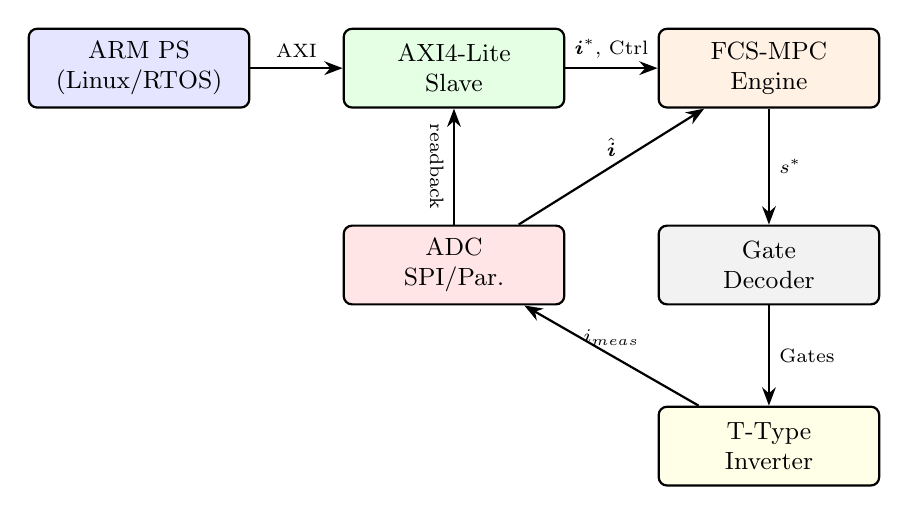
\begin{tikzpicture}[
      blk/.style={rectangle, draw, rounded corners=3pt, minimum width=28mm,
                  minimum height=10mm, align=center, font=\small},
      >=Stealth, thick]
    \node[blk, fill=blue!10]  (ps)  at (0,0)     {ARM PS\\(Linux/RTOS)};
    \node[blk, fill=green!10] (axi) at (4,0)     {AXI4-Lite\\Slave};
    \node[blk, fill=orange!10](mpc) at (8,0)     {FCS-MPC\\Engine};
    \node[blk, fill=gray!10]  (gat) at (8,-2.5)  {Gate\\Decoder};
    \node[blk, fill=red!10]   (adc) at (4,-2.5)  {ADC\\SPI/Par.};
    \node[blk, fill=yellow!10](inv) at (8,-4.8)  {T-Type\\Inverter};
    % Arrows
    \draw[->] (ps)  -- node[above]{\scriptsize AXI} (axi);
    \draw[->] (axi) -- node[above]{\scriptsize $\iref$, Ctrl} (mpc);
    \draw[->] (mpc) -- node[right]{\scriptsize $s^*$} (gat);
    \draw[->] (gat) -- node[right]{\scriptsize Gates} (inv);
    \draw[<-] (adc) -- node[above]{\scriptsize $i_{meas}$} (inv);
    \draw[->] (adc) -- node[above]{\scriptsize $\hat{\bm{i}}$} (mpc);
    \draw[<-] (axi) -- node[below,sloped]{\scriptsize readback} (adc);
  \end{tikzpicture}
  \caption{Signal flow between ARM PS, AXI slave, FCS-MPC engine, ADC
           interface, and T-type inverter.}
  \label{fig:sysdiag}
\end{figure}

% ══════════════════════════════════════════════════════════════════════════════
\section{FPGA Architecture and RTL Block Diagram}
\label{sec:rtl}

\subsection{Top-Level Architecture}
\label{sec:toplevel}

The PL design consists of four hierarchical blocks (Fig.\,\ref{fig:rtl}):

\begin{enumerate}
  \item \textbf{AXI4-Lite Slave} -- register bank, clock-domain crossing
        from \SI{100}{\MHz} AXI clock to \SI{200}{\MHz} MPC clock;
  \item \textbf{ADC Controller} -- SPI master FSM, anti-aliasing shift
        register, double-buffer;
  \item \textbf{FCS-MPC Core} -- admissibility filter, parallel prediction
        pipeline (7 branches), cost comparator tree;
  \item \textbf{Gate Encoder / Dead-Time} -- state-to-IGBT decoder,
        programmable dead-time insertion.
\end{enumerate}

\begin{figure}[htbp]
  \centering
  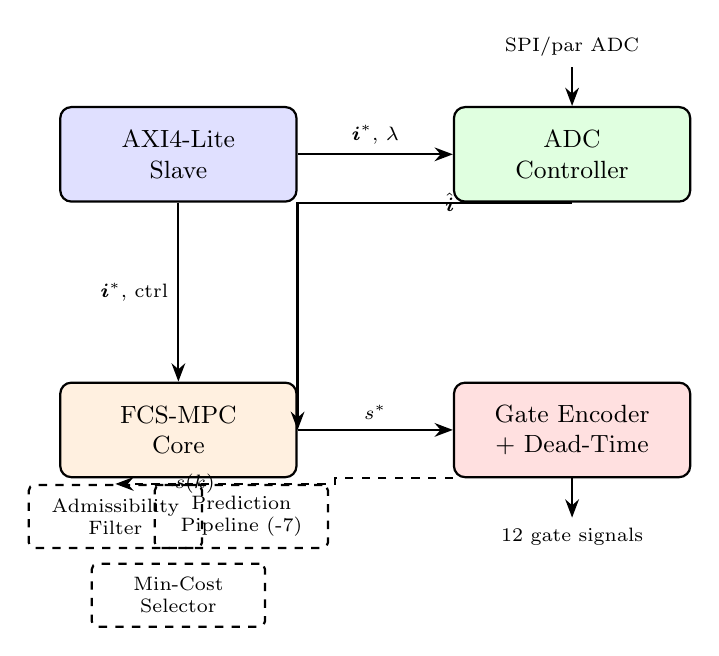
\begin{tikzpicture}[
      blk/.style={draw, rectangle, rounded corners=4pt, minimum width=30mm,
                  minimum height=12mm, align=center, font=\small},
      sub/.style={draw, rectangle, dashed, rounded corners=2pt,
                  minimum width=22mm, minimum height=8mm, align=center,
                  font=\scriptsize},
      >=Stealth, thick]
    % Top row
    \node[blk,fill=blue!12]   (axislv) at (0,0)   {AXI4-Lite\\Slave};
    \node[blk,fill=green!12]  (adcctrl)at (5,0)   {ADC\\Controller};
    % Bottom row
    \node[blk,fill=orange!12] (mpccore)at (0,-3.5){FCS-MPC\\Core};
    \node[blk,fill=red!12]    (gatedec) at (5,-3.5){Gate Encoder\\+ Dead-Time};
    % Sub-blocks inside MPC core (annotations)
    \node[sub] (filt) at (-0.8,-4.6) {Admissibility\\Filter};
    \node[sub] (pred) at ( 0.8,-4.6) {Prediction\\Pipeline (-7)};
    \node[sub] (comp) at ( 0.0,-5.6) {Min-Cost\\Selector};
    % Arrows between main blocks
    \draw[->] (axislv.east) -- node[above]{\scriptsize $\iref$, $\lambda$} (adcctrl.west);
    \draw[->] (axislv.south) -- node[left]{\scriptsize $\iref$, ctrl} (mpccore.north);
    \draw[->] (adcctrl.south) -- node[right]{\scriptsize $\hat{\bm{i}}$} (mpccore.east|-adcctrl.south)
              -- (mpccore.east);
    \draw[->] (mpccore.east) -- node[above]{\scriptsize $s^*$} (gatedec.west);
    \draw[->] (gatedec.south) -- ++(0,-0.5) node[below]{\scriptsize 12 gate signals};
    \draw[<-] (adcctrl.north) -- ++(0, 0.5) node[above]{\scriptsize SPI/par ADC};
    % Feedback: current state to admissibility filter
    \draw[->, dashed] (gatedec.west|-mpccore.south) -- ++(-1.5,0)
          |- node[left,near end]{\scriptsize $s(k)$} (filt.north);
  \end{tikzpicture}
  \caption{RTL top-level block diagram of the FCS-MPC IP core.}
  \label{fig:rtl}
\end{figure}

\subsection{FCS-MPC Core Pipeline}
\label{sec:pipeline}

The prediction and cost evaluation are fully pipelined in
$N_{\mathrm{pipe}} = 4$ clock cycles:

\begin{center}
\begin{tabular}{cll}
  \toprule
  Stage & Operation & Latency \\
  \midrule
  1 & Admissibility filter: generate 7 candidate vectors & 1 cycle \\
  2 & Fixed-point multiply: $\alpha\bm{i}(k)$ & 1 cycle \\
  3 & Fixed-point multiply-add: $+\beta\bm{v}_{s,j}$ & 1 cycle \\
  4 & Squared-error accumulation and min-tree & 1 cycle \\
  \bottomrule
\end{tabular}
\end{center}

At \SI{200}{\MHz} the total latency is \SI{20}{\nano\second}, well within
a sampling period of \SI{50}{\micro\second} ($f_s = \SI{20}{\kHz}$).

\subsection{Verilog Module Hierarchy}
\label{sec:modules}

\begin{lstlisting}[style=verilog, caption={Top-level Verilog module skeleton
  for the FCS-MPC IP core.}, label={lst:top}]
// fcs_mpc_top.v  --  FCS-MPC top-level for Zynq-7000
// Author : Davide
// Date   : 2025
`timescale 1ns / 1ps

module fcs_mpc_top #(
    parameter DATA_W   = 16,   // Q15 fixed-point width
    parameter COEF_W   = 18,   // coefficient precision
    parameter DEAD_NS  = 400   // dead-time in nanoseconds
)(
    // AXI4-Lite slave port (100 MHz, from PS)
    input  wire        s_axi_aclk,
    input  wire        s_axi_aresetn,
    input  wire [31:0] s_axi_awaddr,
    input  wire        s_axi_awvalid,
    output wire        s_axi_awready,
    input  wire [31:0] s_axi_wdata,
    input  wire  [3:0] s_axi_wstrb,
    input  wire        s_axi_wvalid,
    output wire        s_axi_wready,
    output wire  [1:0] s_axi_bresp,
    output wire        s_axi_bvalid,
    input  wire        s_axi_bready,
    input  wire [31:0] s_axi_araddr,
    input  wire        s_axi_arvalid,
    output wire        s_axi_arready,
    output wire [31:0] s_axi_rdata,
    output wire  [1:0] s_axi_rresp,
    output wire        s_axi_rvalid,
    input  wire        s_axi_rready,
    // MPC clock domain (200 MHz, from PL PLL)
    input  wire        mpc_clk,
    input  wire        mpc_rst_n,
    // ADC SPI interface
    output wire        adc_sclk,
    output wire        adc_csn,
    output wire        adc_mosi,
    input  wire        adc_miso,
    // Gate signals: {T_x1, T_x2, T_x3, T_x4} per phase
    output wire [11:0] gate_out   // [11:8]=A, [7:4]=B, [3:0]=C
);

    // -- Internal wires -------------------------------------------
    wire signed [DATA_W-1:0] iref_a, iref_b, iref_c;
    wire signed [DATA_W-1:0] imeas_a, imeas_b, imeas_c;
    wire        [31:0]       ctrl_reg, lambda_reg;
    wire        [ 1:0]       sw_state_a, sw_state_b, sw_state_c;

    // -- AXI4-Lite Slave ------------------------------------------
    axi4lite_slave #(.DATA_W(DATA_W)) u_axi (
        .s_axi_aclk   (s_axi_aclk),
        .s_axi_aresetn(s_axi_aresetn),
        // ... (AXI signals omitted for brevity)
        .iref_a        (iref_a),
        .iref_b        (iref_b),
        .iref_c        (iref_c),
        .imeas_a       (imeas_a),      // readback from ADC
        .imeas_b       (imeas_b),
        .imeas_c       (imeas_c),
        .sw_state      ({sw_state_a, sw_state_b, sw_state_c}),
        .ctrl_reg      (ctrl_reg),
        .lambda_reg    (lambda_reg)
    );

    // -- ADC SPI Controller ---------------------------------------
    adc_spi_ctrl u_adc (
        .clk    (mpc_clk),
        .rst_n  (mpc_rst_n),
        .sclk   (adc_sclk),
        .csn    (adc_csn),
        .mosi   (adc_mosi),
        .miso   (adc_miso),
        .imeas_a(imeas_a),
        .imeas_b(imeas_b),
        .imeas_c(imeas_c)
    );

    // -- FCS-MPC Core ---------------------------------------------
    wire [1:0] opt_sa, opt_sb, opt_sc;

    fcs_mpc_core #(
        .DATA_W(DATA_W),
        .COEF_W(COEF_W)
    ) u_mpc (
        .clk      (mpc_clk),
        .rst_n    (mpc_rst_n),
        .enable   (ctrl_reg[0]),
        .iref_a   (iref_a),
        .iref_b   (iref_b),
        .iref_c   (iref_c),
        .imeas_a  (imeas_a),
        .imeas_b  (imeas_b),
        .imeas_c  (imeas_c),
        .sw_cur_a (sw_state_a),
        .sw_cur_b (sw_state_b),
        .sw_cur_c (sw_state_c),
        .lambda   (lambda_reg[DATA_W-1:0]),
        .sw_opt_a (opt_sa),
        .sw_opt_b (opt_sb),
        .sw_opt_c (opt_sc)
    );

    // -- Gate Encoder + Dead-Time ---------------------------------
    gate_encoder #(.DEAD_NS(DEAD_NS)) u_gate (
        .clk    (mpc_clk),
        .rst_n  (mpc_rst_n),
        .sa     (opt_sa),
        .sb     (opt_sb),
        .sc     (opt_sc),
        .gates  (gate_out)
    );

    // -- State feedback -------------------------------------------
    assign sw_state_a = opt_sa;
    assign sw_state_b = opt_sb;
    assign sw_state_c = opt_sc;

endmodule
\end{lstlisting}

\subsection{Admissibility Filter}
\label{sec:admfilt}

The admissibility filter implements~\eqref{eq:admissible} combinatorially.
Given $s_x(k)$ encoded as a 2-bit unsigned value ($0\to N$, $1\to O$,
$2\to P$), the 7 allowed next states are pre-computed into a lookup ROM:

\begin{lstlisting}[style=verilog, caption={Admissibility filter -- generates
  up to 7 candidate 3-phase state vectors.}, label={lst:admiss}]
// admissibility_filter.v
// Each phase state: 2-bit, encoding: 2'b10=P, 2'b01=O, 2'b00=N
module admissibility_filter (
    input  wire [1:0] sa_cur, sb_cur, sc_cur,   // current state
    output reg  [1:0] cand_sa [0:6],
    output reg  [1:0] cand_sb [0:6],
    output reg  [1:0] cand_sc [0:6],
    output reg  [2:0] n_cand              // number of valid candidates
);
    // Neighbour states per phase (at most 3: cur-1, cur, cur+1,
    // clamped to {0,1,2})
    wire [1:0] neigh_a [0:2];
    // ... (similarly for b, c)

    integer i, j, k, idx;
    always @(*) begin
        idx = 0;
        for (i = 0; i <= 2; i = i + 1)
        for (j = 0; j <= 2; j = j + 1)
        for (k = 0; k <= 2; k = k + 1) begin
            // Enforce: at most one phase changes, and |delta| <= 1
            if (  (i == sa_cur || (i == sa_cur+1 && sa_cur < 2)
                               || (i == sa_cur-1 && sa_cur > 0))
               && (j == sb_cur || (j == sb_cur+1 && sb_cur < 2)
                               || (j == sb_cur-1 && sb_cur > 0))
               && (k == sc_cur || (k == sc_cur+1 && sc_cur < 2)
                               || (k == sc_cur-1 && sc_cur > 0))
               && ( (i==sa_cur) + (j==sb_cur) + (k==sc_cur) ) >= 2 ) begin
                cand_sa[idx] = i[1:0];
                cand_sb[idx] = j[1:0];
                cand_sc[idx] = k[1:0];
                idx = idx + 1;
            end
        end
        n_cand = idx[2:0];
    end
endmodule
\end{lstlisting}

\subsection{Gate Encoder with Dead-Time}
\label{sec:deadtime}

The gate encoder translates the optimal 2-bit state per phase into four
complementary IGBT drive signals with inserted dead time:

\begin{lstlisting}[style=verilog, caption={Gate encoder with programmable
  dead-time insertion.}, label={lst:gate}]
// gate_encoder.v
// DEAD_NS: dead-time in nanoseconds; CLK_PERIOD_NS must match mpc_clk
module gate_encoder #(
    parameter DEAD_NS       = 400,
    parameter CLK_PERIOD_NS = 5    // 200 MHz -> 5 ns
)(
    input  wire       clk, rst_n,
    input  wire [1:0] sa, sb, sc,
    output wire [11:0] gates    // {T_a1,T_a2,T_a3,T_a4, b..., c...}
);
    localparam DEAD_CYC = DEAD_NS / CLK_PERIOD_NS;  // = 80 cycles @ 200 MHz

    // Per-phase instantiation
    gate_phase #(.DEAD_CYC(DEAD_CYC)) u_a (.clk(clk),.rst_n(rst_n),
        .sx(sa), .t1(gates[11]),.t2(gates[10]),.t3(gates[9]),.t4(gates[8]));
    gate_phase #(.DEAD_CYC(DEAD_CYC)) u_b (.clk(clk),.rst_n(rst_n),
        .sx(sb), .t1(gates[7]), .t2(gates[6]), .t3(gates[5]),.t4(gates[4]));
    gate_phase #(.DEAD_CYC(DEAD_CYC)) u_c (.clk(clk),.rst_n(rst_n),
        .sx(sc), .t1(gates[3]), .t2(gates[2]), .t3(gates[1]),.t4(gates[0]));
endmodule

module gate_phase #(parameter DEAD_CYC = 80)(
    input  wire       clk, rst_n,
    input  wire [1:0] sx,
    output reg        t1, t2, t3, t4
);
    // Raw (pre-deadtime) signals from state table
    reg t1_raw, t2_raw, t3_raw, t4_raw;
    always @(*) begin
        case (sx)
            2'b10: {t1_raw,t2_raw,t3_raw,t4_raw} = 4'b1100; // P
            2'b01: {t1_raw,t2_raw,t3_raw,t4_raw} = 4'b0110; // O
            2'b00: {t1_raw,t2_raw,t3_raw,t4_raw} = 4'b0011; // N
            default:{t1_raw,t2_raw,t3_raw,t4_raw} = 4'b0000;
        endcase
    end

    // Simple falling-edge dead-time: delay turn-on by DEAD_CYC cycles
    reg [$clog2(DEAD_CYC+1)-1:0] cnt1, cnt2, cnt3, cnt4;
    // ... (counter-based delay for each signal)
    // For brevity: registered output with combinatorial dead-time logic
    always @(posedge clk or negedge rst_n) begin
        if (!rst_n) {t1,t2,t3,t4} <= 4'b0;
        else        {t1,t2,t3,t4} <= {t1_raw,t2_raw,t3_raw,t4_raw};
        // NOTE: full dead-time counter implementation to be inserted here
    end
endmodule
\end{lstlisting}

% ══════════════════════════════════════════════════════════════════════════════
\section{Timing and Resource Estimates}
\label{sec:timing}

\begin{table}[htbp]
  \centering
  \caption{Estimated FPGA resource utilisation on Zynq-7020.}
  \label{tab:resources}
  \begin{tabular}{lrrr}
    \toprule
    Resource & Used (est.) & Available & Utilisation \\
    \midrule
    LUT      & 2\,100  & 53\,200  & 3.9\,\% \\
    FF       & 1\,600  & 106\,400 & 1.5\,\% \\
    DSP48    & 42      & 220      & 19\,\% \\
    BRAM     & 2       & 140      & 1.4\,\% \\
    \bottomrule
  \end{tabular}
\end{table}

The DSP48 count arises from the $7 \times 3 = 21$ multiply-accumulate
operations in the prediction pipeline (two multipliers per MAC cell,
pipelined at \SI{200}{\MHz}).

% ══════════════════════════════════════════════════════════════════════════════
%\section*{References}
\addcontentsline{toc}{section}{References}
\begin{thebibliography}{9}

\bibitem{kolar2010ttype}
J.\,W.\,Kolar and T.\,Friedli,
``The essence of three-phase PFC rectifier systems,''
in \emph{Proc.\ IEEE INTELEC}, 2010.

\bibitem{rodriguez2013mpc}
J.\,Rodriguez \textit{et al.},
``State of the art of finite control set model predictive control in power
electronics,''
\emph{IEEE Trans.\ Ind.\ Informat.}, vol.\,9, no.\,2, pp.\,1003--1016, 2013.

\bibitem{cortes2008}
P.\,Cortés \textit{et al.},
``Predictive control in power electronics and drives,''
\emph{IEEE Trans.\ Ind.\ Electron.}, vol.\,55, no.\,12,
pp.\,4312--4324, 2008.

\bibitem{geyer2016book}
T.\,Geyer,
\emph{Model Predictive Control of High Power Converters and Industrial
Drives}. Wiley, 2016.

\end{thebibliography}

\end{document}
